\iffalse
\documentclass[12pt]{article}
\usepackage{graphicx}
\usepackage{commath}
\usepackage{gensymb}
\usepackage{float}

\begin{document}
\begin{center}
\textbf\large{CHAPTER-7 \\ COORDINATE GEOMETRY}
\end{center}

\section{EXERCISE - 7.1}
\fi
\begin{enumerate}[label=\thesection.\arabic*,ref=\thesection.\theenumi]
\numberwithin{equation}{enumi}
\numberwithin{figure}{enumi}
\numberwithin{table}{enumi}
\item Find the distances between the following pairs of points:
\begin{enumerate}
\item $(2,3),(4,1)$
\item $(-5,7),(-1,3)$
\item $(a,b),(-a,-b)$
\end{enumerate}
\item Find the distance between the points $(0,0)$ and $ (36,15)$.
\item Determine if the points $(1,5),(2,3)$ and $(-2,-11)$ are collinear.
	\\
		\iffalse
\documentclass[12pt]{article}
\usepackage{graphicx}
\usepackage[none]{hyphenat}
\usepackage{graphicx}
\usepackage{listings}
\usepackage[english]{babel}
\usepackage{graphicx}
\usepackage{caption} 
\usepackage{hyperref}
\usepackage{booktabs}
\usepackage{array}
\usepackage{amsmath}   % for having text in math mode
\usepackage{extarrows} % for Row operations arrows
\usepackage{listings}
\lstset{
  frame=single,
  breaklines=true
}
  
%Following 2 lines were added to remove the blank page at the beginning
\usepackage{atbegshi}% http://ctan.org/pkg/atbegshi
\AtBeginDocument{\AtBeginShipoutNext{\AtBeginShipoutDiscard}}


%New macro definitions
\newcommand{\mydet}[1]{\ensuremath{\begin{vmatrix}#1\end{vmatrix}}}
\providecommand{\brak}[1]{\ensuremath{\left(#1\right)}}
\providecommand{\norm}[1]{\left\lVert#1\right\rVert}
\newcommand{\solution}{\noindent \textbf{Solution: }}
\newcommand{\myvec}[1]{\ensuremath{\begin{pmatrix}#1\end{pmatrix}}}
\let\vec\mathbf

\begin{document}

\begin{center}
\title{\textbf{Properties of Triangles}}
\date{\vspace{-5ex}} %Not to print date automatically
\maketitle
\end{center}
\setcounter{page}{1}

\section{10$^{th}$ Maths - Chapter 7}
This is Problem-3 from Exercise 7.1
\begin{enumerate}
\item Determine if the points $(1,5), (2,3), \text{ and } (-2,-11)$ are collinear.  \\
	\fi
\solution 
 We know that points $\vec{A}, \vec{B} \text{ and } \vec{C}$ are collinear, if
\begin{align}
  \label{eq:10/7/1/31}
\text{rank}\myvec{ 
	\vec{A}^\top \\ 
	\vec{B}^\top \\ 
	\vec{C}^\top 
}    &=  1 
\end{align}
Since
\begin{align}
	\myvec{ \vec{A}^\top \\ 
			\vec{B}^\top \\ 
			\vec{C}^\top 
} =   		\myvec{
        		1 & 5 \\
        		2 & 3 \\
        		-2 & -11 
}
\\
\xleftrightarrow[{R_3\rightarrow R_3+2R_1}]{{R_2\rightarrow R_2-2R_1}}  \myvec{
  1 & 5 \\
  0 & -7 \\
  0 & -1 
}    
\xleftrightarrow[]{{R_3\rightarrow R_3-\frac{1}{7}R_2}}  \myvec{
  1 & 5 \\
  0 & -7 \\
  0 & 0 
},
\end{align}
 the rank of the matrix is 2. From \eqref{eq:10/7/1/31}, the points are not collinear.  This is verified by Fig.  
 \ref{fig:10/7/1/3Fig1}, where the given points constitute a triangle and not a line.
\begin{figure}[!h]
	\begin{center}
		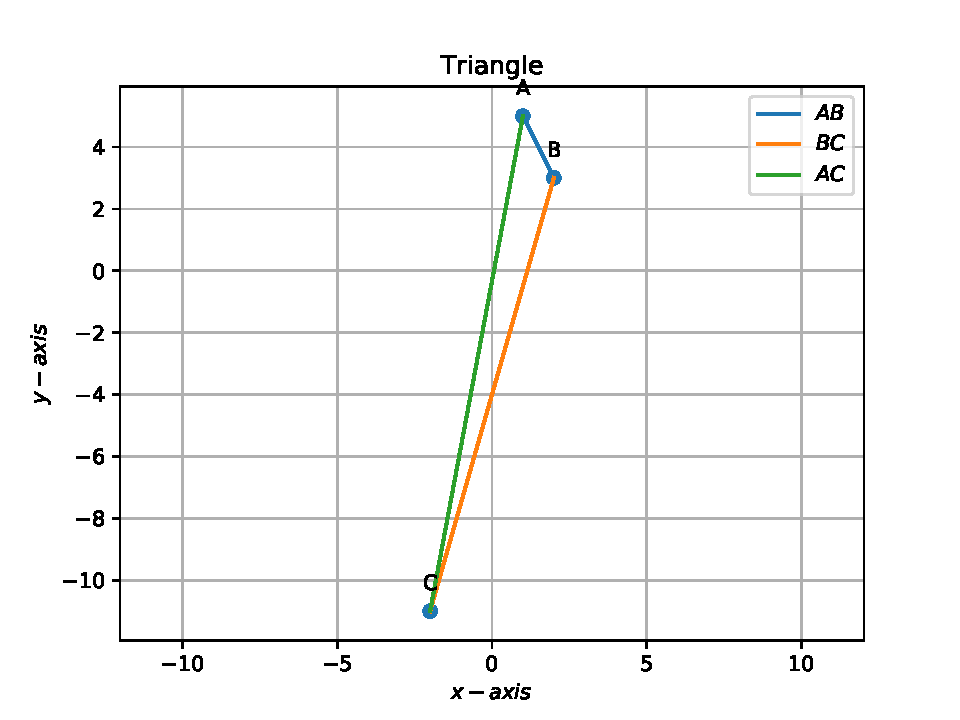
\includegraphics[width=\columnwidth]{chapters/10/7/1/3/figs/problem3.pdf}
	\end{center}
\caption{}
\label{fig:10/7/1/3Fig1}
\end{figure}


\item Check whether$(5,-2),(6,4)$ and $(7,-2)$ are the vertices of an isosceles triangle.
	\iffalse
\item  In a classroom, 4 friends are seated at the points A,B,C and D as shown in Fig. 7.8, Champa and Chameli walk in to the class and after observing for a few minutes Champa asks Chameli,"Dont't you think ABCD is a square?" Chameli disagrees,Using distance formula, find which of them is correct.

\begin{figure}[!h]
\centering
  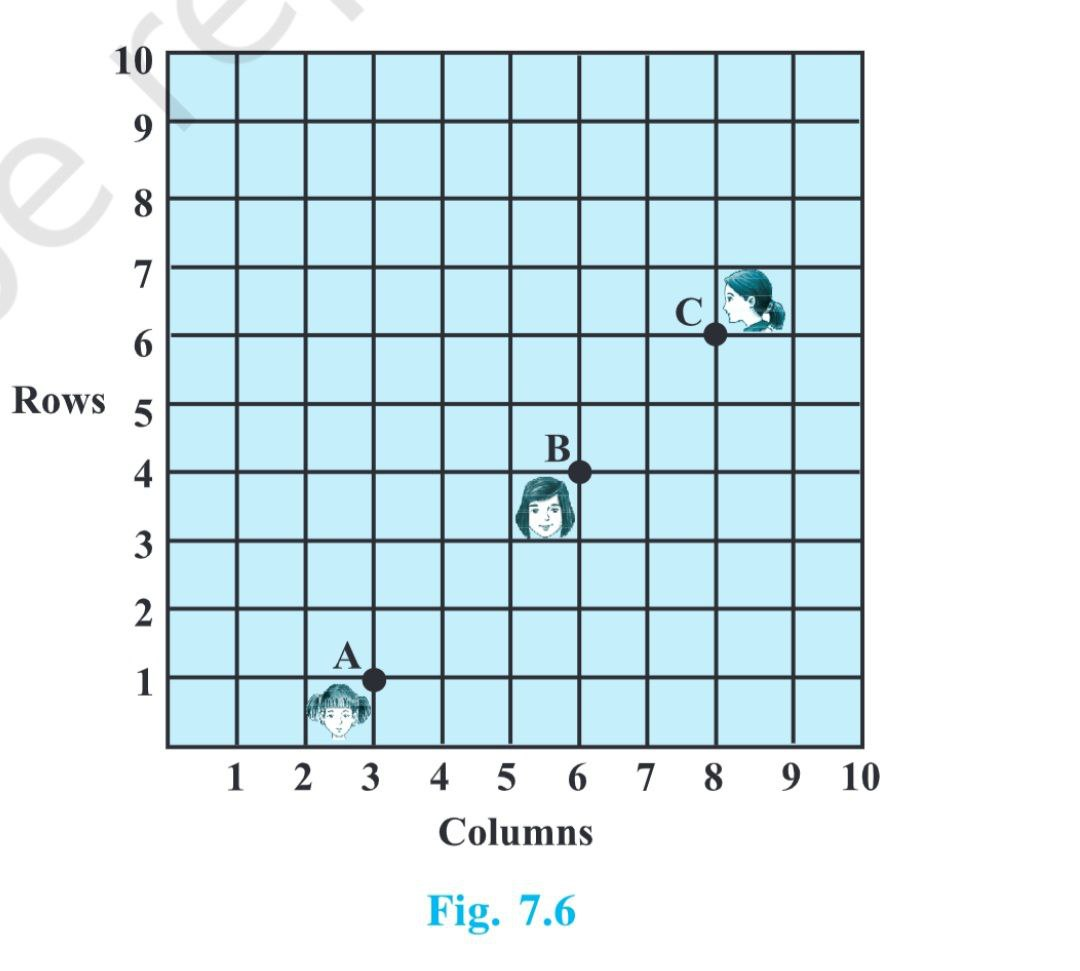
\includegraphics[width=\columnwidth]{canvas.jpg}
 \caption{}
\label{fig:10/7/4/8Fig3}
\end{figure}
\fi
\item Name the type of quadrilateral formed,if any,by the following points,and give reasons for your answer
\begin{enumerate}
\item $(-1,-2),(1,0),(-1,2),(-3,0)$
\item $(-3,5),(-3,1),(0,3),(-1,-4)$
\item $(4,5),(7,6),(4,3),(1,2)$
\end{enumerate}
\solution
		\iffalse
\documentclass[12pt]{article}
\usepackage{graphicx}
\usepackage{amsmath}
\usepackage{mathtools}
\usepackage{gensymb}

\newcommand{\mydet}[1]{\ensuremath{\begin{vmatrix}#1\end{vmatrix}}}
\providecommand{\brak}[1]{\ensuremath{\left(#1\right)}}
\providecommand{\norm}[1]{\left\lVert#1\right\rVert}
\newcommand{\solution}{\noindent \textbf{Solution: }}
\newcommand{\myvec}[1]{\ensuremath{\begin{pmatrix}#1\end{pmatrix}}}
\let\vec\mathbf

\begin{document}
\begin{center}
\textbf\large{CHAPTER-7 \\ COORDINATE GEOMETRY}

\end{center}
\section*{Excercise 7.1}

Q6.Name the type of quadilateral formed,if any, by the following points, and give reasons for your answer:
\begin{enumerate}
	\item $\brak{-1,-2}, \brak{1,0}, \brak{-1,2}, \brak{-3,0}$ 
	\item $\brak{-3,5}, \brak{3,1}, \brak{0,3}, \brak{-1,-4}$
	\item $\brak{4,5}, \brak{7,6}, \brak{4,3}, \brak{1,2}$
\end{enumerate}
\solution
\fi
\begin{enumerate}
\item The coordinates are given as
	\begin{align}
	\vec{A} = \myvec{
		-1\\
		-2\\
		},
	\vec{B} = \myvec{
		1\\
		0\\
		},
	\vec{C} = \myvec{
		-1\\
		2\\
		} \text{ and }
	\vec{D} = \myvec{
		-3\\
		0\\
		}
	\end{align}
	\begin{align}
		\vec{B} - \vec{A} &= \myvec{1\\0} - \myvec{-1\\-2} = \myvec{2\\2}\\
		\vec{C} - \vec{B} &= \myvec{-1\\2} - \myvec{1\\0} = \myvec{-2\\2}\\
		\vec{C} - \vec{D} &= \myvec{-1\\2} - \myvec{-3\\0} = \myvec{2\\2}\\
		\vec{D} - \vec{A} &= \myvec{-3\\0} - \myvec{-1\\-2} = \myvec{-2\\2}
	\end{align}
	\begin{align}	
		\vec{C} - \vec{A} &= \myvec{-1\\2} - \myvec{-1\\-2} = \myvec{0\\4}\\
		\vec{D} - \vec{B} &= \myvec{-3\\0} - \myvec{1\\0} = \myvec{-4\\0}
	\end{align}
	\begin{align}	
		\vec{B}-\vec{A} = \vec{C}-\vec{D} \text{ and } \vec{C}-\vec{B} = \vec{D}-\vec{A}.
	\end{align}
	Hence, $ABCD$ is a parallelogram.
	\begin{enumerate}
		\item Now checking if the adjacent sides are orthogonal to each other
	\begin{align}
		(\vec{B}-\vec{A})^\top (\vec{C}-\vec{B}) = \myvec{2&2} \myvec{-2\\2} = -4+4 = 0
	\end{align}
		\item Now checking if the diagonals are also orthogonal then it is a square else a rectangle.
	\end{enumerate}	
	\begin{align}
		(\vec{C}-\vec{A})^\top (\vec{D}-\vec{B}) = \myvec{0&4} \myvec{-4\\0} = 0
	\end{align}
	Hence the diagonals are orthogonal to each other.

	So, we can conclude that $ABCD$ is a square.

	As shown in Figure \ref{fig:10/7/1/6/Fig1} we can see that $ABCD$ is a square hence we can conclude that our theoritical result is verified.
 
\begin{figure}[!h]
	\begin{center} 
	    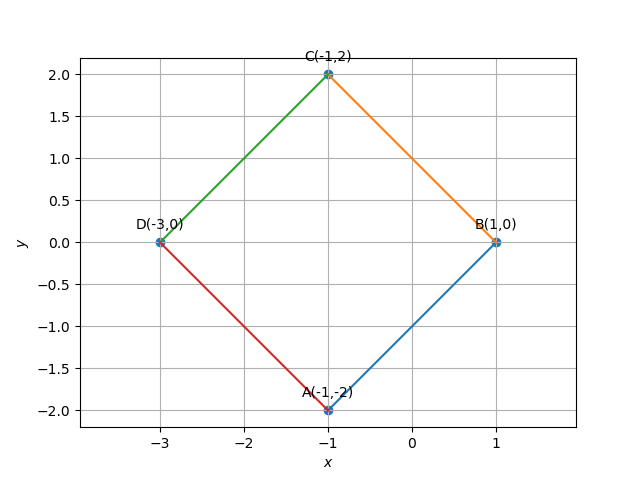
\includegraphics[width=\columnwidth]{chapters/10/7/1/6/figs/quad1}
	\end{center}
\caption{}
\label{fig:10/7/1/6/Fig1}
\end{figure}

\item The coordinates are given as
	\begin{align}
	\vec{A} = \myvec{
		-3\\
		5\\
		},
	\vec{B} = \myvec{
		3\\
		1\\
		},
	\vec{C} = \myvec{
		0\\
		3\\
		} \text{ and }
	\vec{D} = \myvec{
		-1\\
		-4\\
		}
	\end{align}
	\begin{align}
		\vec{B} - \vec{A} &= \myvec{3\\1} - \myvec{-3\\5} = \myvec{6\\-4}\\
		\vec{C} - \vec{B} &= \myvec{0\\3} - \myvec{3\\1} = \myvec{-3\\2}\\
		\vec{C} - \vec{D} &= \myvec{0\\3} - \myvec{-1\\-4} = \myvec{1\\7}\\
		\vec{D} - \vec{A} &= \myvec{-1\\-4} - \myvec{-3\\5} = \myvec{2\\-9}
	\end{align}
	\begin{align}
		\vec{C} - \vec{A} &= \myvec{0\\3} - \myvec{-3\\5} = \myvec{3\\-2}\\
		\vec{D} - \vec{B} &= \myvec{-1\\-4} - \myvec{3\\1} = \myvec{-4\\-5}
	\end{align}
	\begin{align}
	\vec{B}-\vec{A} \neq \vec{C}-\vec{D} \text{ and } \vec{C}-\vec{B} \neq \vec{D}-\vec{A},
	\end{align}
	Hence, $ABCD$ is not a parallelogram, it can be a irregular quadilateral.
	\begin{enumerate}
		\item Now to check if any three points are collinear,

	if rank of $\myvec{\vec{B}-\vec{A} & \vec{C}-\vec{B}} = 1$ then points are collinear

	Forming the collinearity matrix
	\begin{align}
		\myvec{6&-3\\-4&2} \xleftrightarrow{R_{2}\rightarrow R_{2}+\frac{2}{3}R_{1}}= \myvec{6&-3\\0&0}
	\end{align}
	\end{enumerate}
	Hence, rank = 1

	Since none of the opposite sides are parallel to each other and three points are collinear so these does not form a quadilateral.

	As shown in Figure \ref{fig:10/7/1/6/Fig2} we can see that $ABCD$ does not form a quadilateral and three points are collinear hence, our theoritical result is verified.
	
\begin{figure}[!h]
	\begin{center} 
	    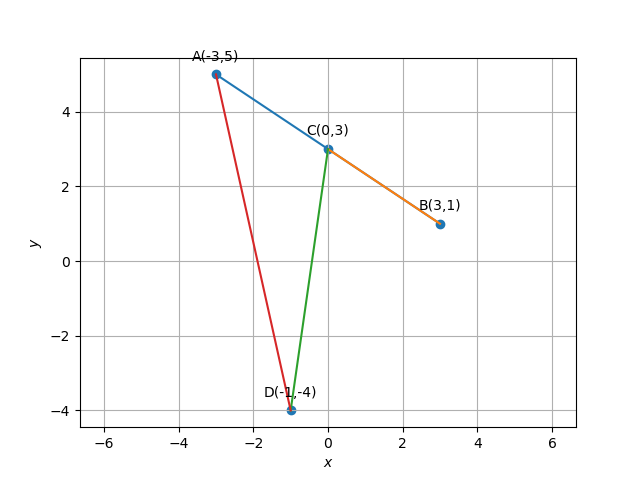
\includegraphics[width=\columnwidth]{chapters/10/7/1/6/figs/quad2}
	\end{center}
\caption{}
\label{fig:10/7/1/6/Fig2}
\end{figure}
	
\item The coordinates are given as
	\begin{align}
	\vec{A} = \myvec{
		4\\
		5\\
		},
	\vec{B} = \myvec{
		7\\
		6\\
		},
	\vec{C} = \myvec{
		4\\
		3\\
		} \text{ and }
	\vec{D} = \myvec{
		1\\
		2\\
		}
	\end{align}
	\begin{align}
		\vec{B} - \vec{A} &= \myvec{7\\6} - \myvec{4\\5} = \myvec{3\\1}\\
		\vec{C} - \vec{B} &= \myvec{4\\3} - \myvec{7\\6} = \myvec{-3\\-3}\\
		\vec{C} - \vec{D} &= \myvec{4\\3} - \myvec{1\\2} = \myvec{3\\1}\\
		\vec{D} - \vec{A} &= \myvec{1\\2} - \myvec{4\\5} = \myvec{-3\\-3}
	\end{align}
	\begin{align}
		\vec{C} - \vec{A} &= \myvec{4\\3} - \myvec{4\\5} = \myvec{0\\-2}\\
		\vec{D} - \vec{B} &= \myvec{1\\2} - \myvec{7\\6} = \myvec{-6\\-4}
	\end{align}
	\begin{align}
		\vec{B}-\vec{A} = \vec{C}-\vec{D} \text{ and } \vec{C}-\vec{B} = \vec{D}-\vec{A},
	\end{align}
	Hence, $ABCD$ is a parallelogram.
	\begin{enumerate}
		\item Now checking if the adjacent sides are orthogonal to each other
	\begin{align}
		(\vec{B}-\vec{A})^\top (\vec{C}-\vec{B}) = \myvec{3&1} \myvec{-3\\-3} = -9-3 = -12
	\end{align}
	Since inner product is not zero so adjacent sides are not orthogonal.

	Hence, we can say that $ABCD$ is neither a rectangle nor a square.

		\item Now checking if the diagonals are orthogonal then it is a Rhombus.
	\begin{align}
		(\vec{C}- \vec{A})^\top (\vec{D}-\vec{B}) = \myvec{0&-2} \myvec{-6\\-4} = 0+8 = 8
	\end{align}
	\end{enumerate}		
	Hence the diagonals are also not orthogonal so we conclude that $ABCD$ is a parallelogram.

	As shown in Figure \ref{fig:10/7/1/6/Fig3} we can see that $ABCD$ forms a parallelogram hence, our theoritical result is verified.

\begin{figure}[!h]
	\begin{center} 
	    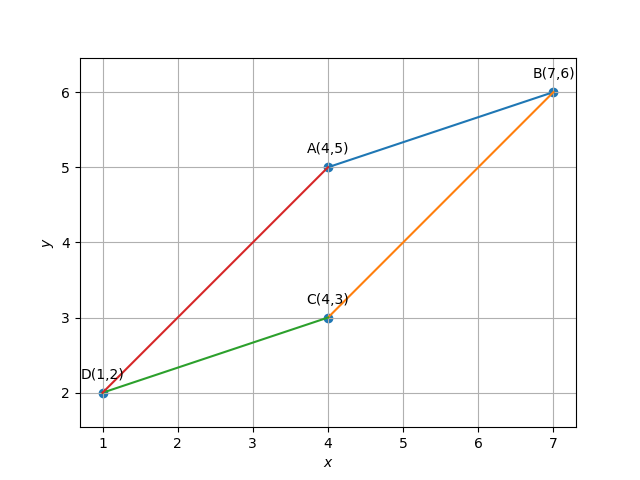
\includegraphics[width=\columnwidth]{chapters/10/7/1/6/figs/quad3}
	\end{center}
\caption{}
\label{fig:10/7/1/6/Fig3}
\end{figure}
\end{enumerate}



\item Find the point on the x-axis which is equidistant from $(2,-5)$ and $(-2,9)$.
\item Find the values of $y$ for which the distance between the points                  $\vec{P}(2,-3)$ and $\vec{Q}(10,y)$ is 10 units.
\item  If $\vec{Q}(0, 1)$ is equidistant from $\vec{P}(5, -3)$ and $\vec{R}(x, 6)$, find the values of $x$. Also find the
distances $QR$ and $PR$.
\item  Find a relation between $x$ and $y$ such that the point $(x,y)$ is equidistant from the point
$(3, 6)$ and $(– 3, 4)$.

\end{enumerate}

